%---------- Segundo Capítulo ----------
\chapter{Mapeamento Sistemático}
\section{Introdução}
%A utilização da arquitetura orientada a serviços (SOA), que consiste em uma coleção de componentes distribuídos que fornecem e ou consomem serviços\cite{Clements2010}, tem sido amplamente utilizada por um grande número de empresas.

%Serviços correspondem a recursos de software bem definidos através de uma linguagem padrão, são auto-contidos,  proveem funcionalidades padrões do negócio, independentes do estado ou contexto de outros serviços \cite{Furtado2009}.

%Nesse contexto a utilização de serviços padronizados tornou-se a solução para a problemática da interoparibilidade entre sistemas, uma vez que permitiu a integração automatizada de negócios entre aplicações.

A utilização da SOA tornou-se uma solução para a problemática da interoperabilidade entre sistemas, uma vez que permitiu a integração automatizada de negócios entre aplicações. Contudo, apesar dos benefícios, existem vários desafios que devem ser considerados quando da implantação de uma arquitetura orientada a serviços~\cite{marks2006}. Dentre eles destaca-se o requisito não funcional de segurança, que deve ser muito bem planejado de forma que o serviço oferecido não seja vulnerável a ameaças que comprometam sua integridade, confidencialidade, disponibilidade e autenticidade. Dessa forma, é de suma importância conhecer e aplicar os mecanismos de segurança em uma Arquitetura Orientada a Serviços.

Com a intenção de identificar trabalhos primários relevantes e reconhecidos, com vistas a aumentar o conhecimento da aplicabilidade de mecanismos de segurança a arquitetura orientada a serviços, fez-se necessário realizar um mapeamento sistemático que identificasse as principais pesquisas que envolvessem o tema segurança em SOA.

%Dentre as alternativas optou-se pelo mapeamento sistemático que tem como finalidade, classificar e agregar à literatura estudos relevantes. Seu foco está na  pesquisa mais ampla e de natureza exploratória, cuja finalidade é fornecer uma visão geral e encontrar evidências de uma área de pesquisa.

\section{Mapeamento Sistemático}

Essa seção descreve os resultados do mapeamento sistemático conduzido, sendo estruturada conforme as diretrizes discutidas em~\cite{Petersen2008}.

%O mapeamento sistemático possibilita verificar e identificar evidências de uma área, por meio de uma revisão ampla de estudos primários \cite{guidelines-2007}. Já a revisão sistemática foca em questões de pesquisa bem definidas, mais específicas, que podem ser respondidas por pesquisa experimental\cite{Kitchenham2010}. A metodologia adotada para a organizar e estruturar este mapeamento seguiu as diretrizes prospostas em \cite{sbcars2013}.

\section{Protocolo de Estudo}

Para a realização do mapeamento sistemático foi definido um protocolo de estudo que contemplasse as questões de pesquisa, a string de busca e os critérios de exclusão e inclusão de artigos. A finalidade deste processo é a de documentar as etapas do mapeamento além de permitir a sua replicação por outros pesquisadores.

\section{Questões de Pesquisa (QP)}

Com a finalidade de identificar as principais contribuições e estudos sobre \ ``Segurança e SOA\ '' a pesquisa toma a vertente mais específica com as questões abaixo:

\begin{enumerate}[ QP1 )]

    \item Quais são os principais veículos que publicam artigos nessa área?
    busca-se verificar quais são os principais veículos que publicam informações sobre segurança em SOA, de forma que seja possível categorizar e verificar onde foram publicadas as contribuições mais significativas.
	
	\item Qual o tipo de contribuição é a mais proposta nas pesquisas realizadas?
    Neste caso, procura-se verificar quais são as principais contribuições de pesquisa, identificando se o tipo da contribuição é uma proposta, solução, avaliação, validação de algum estudo ou um artigo de opinião.


	\item Quais atributos de segurança são mais abordados nos estudos? Objetiva-se identificar dentre os atributos privacidade, confidencialidade, autenticidade e disponibilidade,  quais são os mais abordados nos estudos categorizados e classificados como solução. Além disso, quando uma solução não for classificada em nenhum desses atributos ele deverá ser classificado como qualidade de serviço. Neste caso, serão classificados os artigos que não se enquadrarem em nenhum dos atributos anteriores, mas que mesmo assim, vise garantir a qualidade de outros atributos que no contexto de segurança em SOA seja relevante. Por exemplo, desempenho e escalabilidade.

    \item Quais contribuições classificadas como solução e categorizadas como: método, técnica ou ferramenta/arquitetura, foram os mais propostos nas pesquisas? Objetiva-se identificar dentre os artigos selecionados e categorizados como Solução quais deles podem ser classificados e quantificados como método, técnica ou ferramenta/arquitetura.



\end{enumerate}

\section{Estratégia de Busca}\label{sec:Obj1}

É oportuno definir uma estratégia de busca para a pesquisa dos estudos primários, sendo necessário determinar as palavras chaves a serem pesquisadas e também onde as buscas serão realizadas~\cite{guidelines-2007}.
A estratégia de busca adotada consistiu objetivamente na busca eletrônica das seguintes bibliotecas digitais:
\begin{enumerate}[ a )]
    \item ACM Digital Library referente aos seguintes periódicos:
       \begin{enumerate}
            \item ACM Transactions on Information and System Security (TISSEC);
            \item ACM Computing Surveys (CSUR).
       \end{enumerate}

    \item IEEE Xplore, apenas por periódicos e
    \item DBLP Computer Science Bibliography nas seguintes conferências:
      \begin{enumerate}
            \item ICWS International Conference on Web Services;
            \item SERVICES;
            \item ARES.
      \end{enumerate}

\end{enumerate}

A opção por essas fontes foi motivada por uma pesquisa inicial realizada na base de dados da DBLP, que retornou 77 publicações. Sendo que após uma análise preliminar, observou-se que as conferências mais relevantes quantitativamente foram as citadas no item c desta seção. Seguiu-se o mesmo procedimento para as bibliotecas citadas nos ítens a e b.

No contexto da elaboração dos termos de busca, para  a base de dados eletrônica, usou-se a abordagem descrita em~\cite{guidelines-2007}, que consiste em criar os termos de busca a partir de questões de pesquisa, usando a composição de operadores AND e OR. Dessa forma, a \emph{string} de busca usada na realização desse estudo foi \textbf{\emph{SOA and SECURITY}} não sendo usados sinônimos ou outras variações.

\section{Critérios de Inclusão e Exclusão}

Após serem realizadas as pesquisas, de acordo com a \emph{string} de busca,  vários estudos primários foram recuperados e avaliados  de forma que fossem  excluídos aqueles que não satisfizessem os objetivos do estudo. A investigação dos estudos consistiu inicialmente em analisar o título, o resumo, a introdução e a conclusão.

As conclusões foram analisadas para entender melhor as contribuições do trabalho. Os critérios de seleção dos estudos foram baseados nas questões de pesquisa e todos os estudos recuperados foram armazenados. Logo, para este mapeamento foram definidos os seguintes critérios de inclusão e exclusão:

No que se refere aos critérios de inclusão, foram incluídos todos os artigos que faziam referência a SOA Security e que foram publicados nos periódicos e conferências publicados no período compreendido do ano de 2000 até 2013 e que satisfizessem a \emph{string} de busca anteriormente definida.

No que tange os critérios de exclusão, foram excluídos os artigos e resumos com menos de quatro páginas, artigos que não tratavam diretamente do tema SOA \emph{SECURITY}, contribuições que, apesar de versar sobre SOA, não faziam referência à segurança e vice-versa, as que tratavam de segurança, mais não tratavam de arquitetura orientada a serviços. Além disso, foram também excluídos os estudos irrelevantes para a pesquisa e aqueles que não puderam ser obtidos gratuitamente.


%\begin{itemize}
    %\item Critérios de Inclusão
      % \begin{enumerate}
       %     \item Foram incluídos todos os artigos que faziam referência a SOA Security e que foram publicados nos periódicos  e conferências   que satisfizessem a string de busca anteriormente definida;
      %      \item Estudos publicados no período compreendido do ano de 2000 até 2013.
       %\end{enumerate}

    % \item Critérios de Exclusão
      %\begin{enumerate}
       %     \item Artigos e resumos com menos de quatro páginas, estudos incompletos e repetidos e apresentações (Power Point);
      %      \item Artigos que não tratavam diretamente do tema SOA SECURITY;
        %    \item Contribuições que, apesar de versar sobre SOA, não faziam referência a segurança e vice-versa, as que tratavam de segurança, mais não tratavam de arquitetura orientada a serviços;
          %  \item Estudos irrelevantes para a pesquisa e aqueles que não puderam ser obtidos pela UNB.

     % \end{enumerate}

%\end{itemize}

\section{Coleta, Armazenamento dos Dados e Análise}

Após a seleção preliminar e seguindo o que foi preconizado na estratégia de busca, foram realizadas buscas automáticas a cada uma das bibliotecas digitais citadas na Seção~\ref{sec:Obj1}, sendo recuperadas ao todo 54 publicações. A última etapa da seleção consistiu em aplicar os critérios de exclusão e inclusão aos artigos selecionados, de forma que se obteve um total de 25 publicações, que foram analisadas e classificadas de acordo com a seguinte classificação:

\begin{enumerate}
            \item Veículos: Neste tópico buscou-se categorizar quais veículos que mais apresentaram publicações;
            \item Pesquisa: Este tópico foi utilizado para definir quais tipos de pesquisa foram propostas no estudo de forma que as publicações foram classificadas como:
                \begin{enumerate}[ a )]
                 \item Solução: Representa as publicações que propõem uma nova técnica, método ou ferramenta/arquitetura e que a partir dela possa ser realizado algum tipo de verificação de viabilidade;

                 \item Validação: Neste caso são proposições de validação de algum estudo que apresente rigor cientifico, tais como estudos empíricos ou provas da aplicação de alguma técnica, podendo ser uma validação formal ou experimental;

                 \item Avaliação: Publicações que apresentaram avaliações comparativas entre técnicas propostas de algum estudo relacionado a Segurança em SOA, sendo  classificado como:

                    \begin{itemize}
                         \item Avaliação Formal, que é aquele que possui detalhes do estudo, sendo possível, caso necessário, realizar uma reprodução do trabalho;

                        \item Avaliação Informal, que é  aquela em que os detalhes do estudo são poucos o que torna difícil sua reprodução;

                        \item Avaliação Preliminar, neste caso serão considerados os estudos cujos resultados podem ser questionados e não apresentam detalhes para reprodução.
                    \end{itemize}


                 \item Artigos de Opinião: que são estudos informais que fazem uma abordagem geral dos aspectos do tema Segurança em SOA.

            \end{enumerate}

            \item Contexto: Busca-se neste tópico classificar as publicações que sejam classificados como uma Solução e possuam atributos  relacionados a segurança em SOA que abordem: privacidade, confidencialidade, autenticidade e disponibilidade.

\end{enumerate}

\section{Resultados}
Nesta seção são descritos os resultados obtidos após o estudo e o mapeamento das principais publicações coletadas na seção 2.5 e que serão utilizados para responder as questões de pesquisas anteriormente definidas.

\subsection{QP 1 \- Questão de Pesquisa 1}

Quais são os principais veículos que publicam artigos nessa área?
Para responder essa pergunta foram analisados os 25 artigos selecionados após a aplicação dos critérios de exclusão e inclusão. Eles foram classificados de acordo com o veículo de publicação do artigo. Essa classificação é apresentada na figura~\ref{fig:grafico_qtd_veiculo}.

\begin{figure}[!htb]
\centering
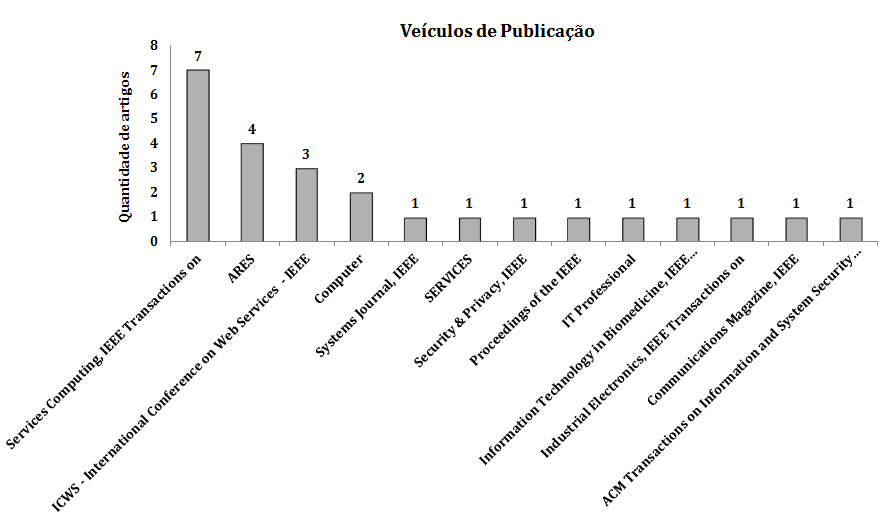
\includegraphics[scale=0.7]{qtd_veiculo_publicacao.png}
\caption{Gráfico representativo da quantidade de contribuições por veículo de publicação.}
\label{fig:grafico_qtd_veiculo}
\end{figure}

Verifica-se que os veículos que mais publicaram artigos relacionados a segurança em SOA foram Services Computing, ARES, ICWS e Computer com 28\%, 16\%, 12\% e 8\% dos artigos publicados, respectivamente. Eles reponderam juntos por aproximadamente 64\% das publicações.

\subsection{QP 2 \- Questão de Pesquisa 2}

Qual o tipo de contribuição é a mais proposta nas pesquisas realizadas?
Após a realização do mapeamento foi possível verificar que dentre os artigos mapeados houve artigos que fizeram referência a mais de um tipo de contribuição. Isso pode ser verificado no artigo proposto por~\cite{Delegation_Solution2011} que foi classificado como sendo uma Solução e uma Validação. Um outro exemplo pode ser observado no artigo~\cite{Vulnerability_Analysis2011} que foi classificado como sendo uma Solução e uma Avaliação. Dessa forma, a contribuição mais proposta foi a Solução com 42\% do total de artigos selecionados, seguidos por Avaliações e Artigos de Opinião ambos com 24\% e finalmente a Validação com 10\%. Dentre essas soluções, cabe ressaltar a que é proposta por~\cite{Vulnerability_Analysis2011}, que propõe um novo método denominado ATLIST, que realiza análise de vulnerabilidades em processos de negócios e serviços baseados em SOA. Este trabalho pode ser útil para a arquitetura de referência que será proposta como resultado deste trabalho de mestrado.

Além desta, outra que também deve ser citada é a que é idealizada por~\cite{Ontology2012}, neste artigo é proposta uma Ontologia, ASSERT4SOA, que foca na interoperabilidade e comparação de certificados heterogêneos e possibilitando a verificação em tempo de execução da conformidade dos serviços com os requisitos de segurança.

Outro artigo relevante para a problemática discutida nesta dissertação é o artigo proposto por~\cite{WeberAM07}. Nesta solução, é proposta uma ferramenta que tem por objetivo identificar possíveis violações de segurança em ambientes SOA. Na ferramenta são descritas formas para inspecionar os arquivos de configuração da plataforma SOA, sendo possível detectar possíveis violações de segurança. Sendo também realizada uma avaliação informal que procura analisar as melhores práticas de segurança em SOA.

Já quanto à contribuição que se refere à avaliação pode-se verificar 4 (quatro) artigos classificados neste tipo, são de avaliações formais, ou seja, estudos que traziam resultados detalhados que podem ser reproduzidos por outros pesquisadores. Um exemplo de avaliação formal pode ser identificado no artigo~\cite{Coetzee2012}. Este artigo analisa os desafios de segurança enfrentados em arquiteturas orientadas a serviço. Os autores propõe uma estrutura de segurança aplicada a SOA baseado em componentes, que consistem em uma variedade de controles que podem minimizar os desafios referentes à aplicação dos mecanismos de segurança em SOA. Os outros artigos classificados como avaliação foram classificados como avaliações informais 4 (quatro) artigos e experimentais 1 (um) artigo totalizando 5 (cinco) artigos.

No que se refere ao tipo de contribuição Validação, foram identificados 4(quatro) artigos  sendo 3(três) validações formais e 1(uma) experimental. Neste tipo de contribuição é relevante citar o trabalho realizado no artigo~\cite{CrossRealmSOA2012}. Neste artigo, é proposta uma ferramenta, que também é uma solução técnica, de um novo protocolo de autenticação para interações de serviços dinâmicos, com base na noção de sessões de negócios multipartidárias orientadas a serviços. Esse protocolo não requer conversão de credencial nem estabelecimento de qualquer caminho de autenticação entre os serviços que participam de uma sessão de negócios. No protocolo são realizadas provas e experimentos para verificar a viabilidade da nova técnica. Este trabalho também poderá ser útil para a arquitetura de referência que será proposta, uma vez que traz uma nova técnica que pode ser utilizada como referência nos processos de autenticação dos serviços oferecidos.

E por fim, no caso dos Artigos de Opinião, foram verificados 9(nove) artigos que faziam uma abordagem geral dos panoramas e desafios de segurança em arquitetura orientada a serviços. Nesses artigos não foi proposto nenhuma contribuição relevante. Porém, como eles se enquadraram nos critérios de busca estabelecidos, foram considerados.

A figura~\ref{fig:Tipo_Contribuicao} apresenta os resultados categorizados pelo tipo da contribuição sendo apresentado o quantitativo de publicações.

\begin{figure}[!htb]
\centering
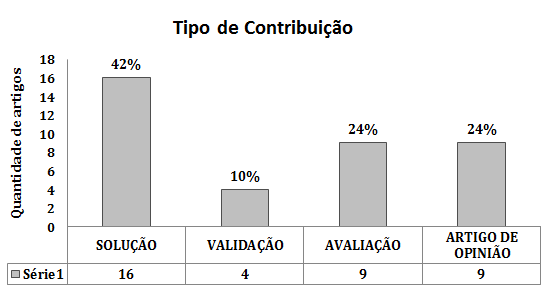
\includegraphics[width=0.8\textwidth]{tipo_contribuicao_3.png}
\caption{Gráfico representativo dos tipos de contribuições}
\label{fig:Tipo_Contribuicao}
\end{figure}


\subsection{QP 3 \- Questão de Pesquisa 3}

Quais atributos de segurança são os mais abordados nos estudos?
Para responder essa pergunta inicialmente realizou-se uma análise nos artigos classificados como Solução. Em seguida foram categorizados de acordo com os atributos relativos à segurança em ambiente SOA. Os atributos analisados foram: integridade, autenticidade, disponibilidade e confidencialidade. Foi possível verificar que dentre os artigos mapeados houve artigos que faziam referência a mais de um atributo. Um exemplo desse fato é descrito na publicação de~\cite{pattern-driven2008} onde são abordados todos os atributos de segurança: integridade, autenticidade, disponibilidade e confidencialidade. Dessa forma, o número de artigos mapeados com os atributos descritos não será equivalente com o número de artigos totalizados no mapeamento.

Sendo assim, o mapeamento identificou que os conceitos mais abordados referem-se aos atributos de autenticidade com 32\% ou 13 artigos e Integridade com 28\% ou 11 artigos. Já o atributo confidencialidade foi verificado em 20\% das publicações, com 8 artigos, e o atributo disponibilidade foi verificado em 15\% das publicações, sendo identificado em 6 artigos. Finalmente, para os artigos que foram classificados como uma solução e que não se enquadraram em nenhum dos atributos, sendo classificados como atributos de qualidade de serviços, foram identificados em apenas 5\% das publicações ou 2 artigos. A Figura~\ref{fig:TipoConceito} apresenta graficamente essa categorização.

\begin{figure}[!htb]
\centering
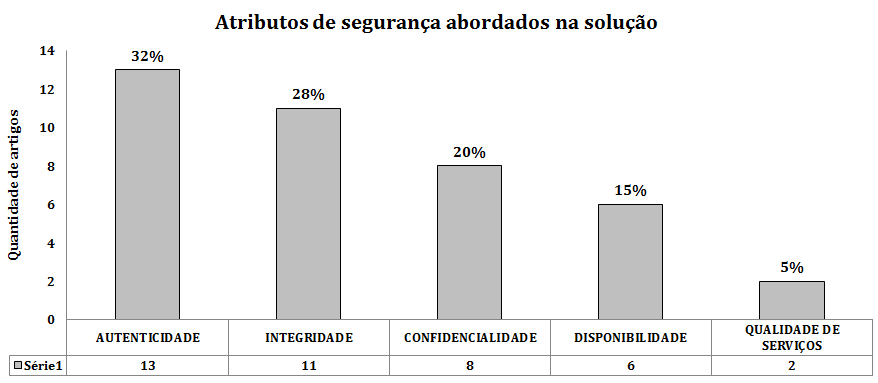
\includegraphics[width=1.0\textwidth]{Atributo_Seguranca_Solucao.png}
\caption{Gráfico dos atributos de segurança abordados na solução}
\label{fig:TipoConceito}
\end{figure}

\subsection{QP 4 \- Questão de Pesquisa 4}

Quais contribuições classificadas como solução e categorizadas como: método, técnica ou ferramenta/arquitetura, foram os mais propostos nas pesquisas?
Para responder essa pergunta, foi realizada uma análise dos artigos classificados como solução. Em seguida foram categorizados de acordo com os tipos: técnica, método ou ferramenta/arquitetura. Verificou-se que entre os artigos mapeados um artigo que fez referência a mais de um tipo de solução.  Esse artigo é descrito na publicação de~\cite{CrossRealmSOA2012} onde são abordados os tipos de solução técnica e ferramenta/arquitetura. Dessa forma, o número de artigos mapeados como sendo uma solução do tipo: método, técnica ou ferramenta/arquitetura não será equivalente com o número de artigos totalizados no mapeamento.

O mapeamento identificou dentre as contribuições classificadas como solução, que o tipo de solução mais proposta é a de solução técnica com 44\% das contribuições ou 7 artigos. As classificadas como ferramenta/arquitetura, foi observado em 31\% das contribuições, ou 5 artigos. Finalmente, o tipo de solução classificado como método, foi verificado em 25\% das contribuições selecionadas, ou 4 artigos. A figura~\ref{fig:TipoConceito} apresenta graficamente essa categorização.


\begin{figure}[!htb]
\centering
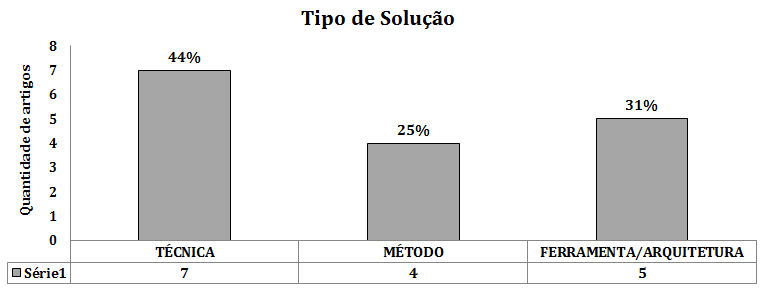
\includegraphics[width=1.0\textwidth]{tipo_solucao.png}
\caption{Gráfico dos tipos de Solução mais propostos}
\label{fig:tipo_solucao}
\end{figure}
%---------- Segundo Capitulo ----------
\subsection{Discussão sobre os Resultados}

De acordo com os resultados obtidos por este mapeamento sistemático foi possível observar que a maioria dos artigos se concentram nos veículos: Services Computing, ARES, ICWS e Computer com 28\%, 16\%, 12\% e 8\%, respectivamente. Eles reponderam juntos por aproximadamente 64\% das publicações.

No que tange os resultados obtidos a respeito do tipo de contribuições, verificou-se que a maior parte de contribuições foram de soluções com 42\% dos artigos e que destas destacaram-se as soluções técnicas com 44\% dos artigos classificados nesta faceta de pesquisa. Este resultado denota que os pesquisadores tem buscado estabelecer padrões e procedimentos  com objetivos específicos de resolver problemas ou melhorar as técnicas existentes que estejam  relacionados a segurança em SOA.

No contexto das contribuições referentes aos atributos de segurança que foram abordados e classificados com solução, verificou-se que as maiores preocupações estavam associadas aos atributos de  autenticidade, integridade e confidencialidade com 33\%, 27\% e 20\% das contribuições respectivamente. Dessa forma, verifica-se que dentre as soluções anteriormente citadas a maior preocupação é em estabelecer técnicas eficientes para autenticar os serviços e garantir que o conteúdo das mensagens não seja modificado. Isso pode denotar uma preocupação com o desempenho dos serviços no momento da aplicação dos mecanismos de segurança.
%
%\subsection{Ameaças a validade}

%As possíveis ameaças aos resultados dessa pesquisa são caracterizados a seguir e seguem  a classificação proposta por \cite{ leedy1980practical} e que foram estruturadas no artigo \cite{sbcars2013}.

\section{Síntese do Capítulo}

O mapeamento sistemático realizado, possibilitou aprofundar os conhecimentos referentes à segurança em SOA. Sendo possível verificar quais são os principais veículos que publicam artigos nesta área, o que ajuda a direcionar os estudos. Também foi possível identificar e analisar quais são os tipos de contribuições que mais são propostas nas pesquisas envolvendo esta temática. Além disso, verificou-se dentre as contribuições propostas como solução, quais delas envolviam atributos de segurança e que tratavam de integridade, autenticidade, disponibilidade e confidencialidade. E por fim, nas contribuições classificadas como solução, foi possível identificar e quantificar quais tipos de solução (método, técnica e ferramentas/arquitetura) foram as mais propostas.

Com este mapeamento sistemático foi possível identificar alguns artigos que serão fundamentais para nortear a pesquisa desenvolvida nesta dissertação. Eles são descritos a seguir:

No artigo~\cite{WeberAM07}, são descritas formas para inspecionar os arquivos de configuração da plataforma SOA, sendo possível detectar possíveis violações de segurança. Um dos focos do trabalho está relacionado com as melhores práticas para a implantação de segurança em SOA, o que pode enriquecer a arquitetura de referência proposta nesta dissertação.

Outro trabalho que também deve ser citado, é o descrito na publicação de~\cite{pattern-driven2008} onde são abordados todos os atributos de segurança: integridade, autenticidade, disponibilidade e confidencialidade. Neste trabalho é proposto uma nova abordagem para proteger aplicativos de SOA. Outro ponto importante, e que a segurança não é considerada como um aspecto isolado, mas como um aspecto presente em todas as fases de um desenvolvimento do sistema.

O artigo descrito em~\cite{Coetzee2012}, analisa os desafios de segurança enfrentados em arquiteturas orientadas a serviço. Sendo proposta uma estrutura de segurança aplicada a SOA, baseado em componentes, que consiste em uma variedade de controles que podem minimizar os desafios referentes à aplicação dos mecanismos de segurança em SOA. Esse artigo realça os desafios de segurança em SOA e pode servir como base para a proposta de criação da arquitetura de referência. 